\section{Problem Statement}%
\label{sec:problem_statement}

\subsection{Toroidal Grid}%
\label{sub:toroidal_grid}


According to the problem description on AZsPCs,\cite{zimmermann} the initial toroidal grid $O$ is defined as an $N\times N$ grid of unique tokens which ``wrap around'' (implications are addressed in \ref{ssub:distance_metric}). These tokens can be arbitrarily defined, as long as they are unique, but for the sake of simplicity (and for reasons explained in \ref{ssub:distance_metric}), in this essay, a token is of the form by $\bm{IJ}$, where $\bm{I}$ and $\bm{J}$ are alphabetic representations of the indices of the rows and columns respectively, of a token, \emph{within $O$}\footnote{This is important because after rearranging the tokens, the identity of the token depends on its position within $O$, and not the rearranged position}, eg.~$AC$ corresponds to the token in row 1, column 3 of $O$, $DF$ corresponds to the row 4, column 6 of $O$, and so on. For $N=4$, the grid is shown in \autoref{fig:toroidExample}. The tokens outside of the square grid represent tokens which wrap around the edges, resembling a toroidal surface as shown in \autoref{fig:wiki_toroid}.
\begin{figure}[htpb]
    \begin{subfigure}[t]{0.5\textwidth}
    \begin{center}
        \raisebox{0.4cm}{
        \includegraphics[width=0.7\textwidth]{images/Simple_Torus.pdf}}
    \caption{A Simple Toroid by Yassine Mrabet\cite{wiki_toroid}}
    \label{fig:wiki_toroid}
    \end{center}
    \end{subfigure}
    ~
    \begin{subfigure}[t]{0.5\textwidth}
    \begin{center}
    \toroidWarp{4}
    \caption{A $4\times 4$ \emph{intial} toroidal grid}%
    \label{fig:toroidExample}
    \end{center}
    \end{subfigure}
    \caption{Representations of a toroidal grid}
\end{figure}


\subsection{Evaluation Function}%
\label{sub:evaluation_function}

The goal of the challenge (and hence this essay) is to create a new grid $X$ --- with tokens rearranged arbitrarily from the initial grid $O$ --- which minimizes a loss function which is computed with the following procedure:
\begin{enumerate}
    \item For each unique pair of tokens\footnote{Comparisons between a token and itself do not affect the loss, since the distance between them is $0$, therefore, their inclusion or exclusion does not affect the computation} (eg. $(AA,BA)$ is equivalent to $(BA,AA)$, so $(BA,AA)$ is excluded), calculate the squared distance between them in the new grid,
    \item Multiply each of them with the squared distance between the pair of tokens within the original grid
    \item The loss is the sum of all of these products
\end{enumerate}

\subsubsection{Distance Metric}%
\label{ssub:distance_metric}
To evaluate the loss function, a distance metric between two tokens must be established. And to do that, we must define the position of a token in a coordinate system. This is where the methodology we used to define the unique tokens comes in handy; the coordinates of the tokens are simply the indices of the token \emph{within the particular grid $X$}. To avoid confusion between whether the rows or columns correspond to the $x$-coordinate or $y$-coordinate, a token within a grid, with indices $(i,j)$ simply has the coordinate $(i,j)$.\footnote{Note that this means we are not adhering to Cartesian coordinates, where the index $(i,j)$ would have the coordinate $(j,i)$.}

With this definition, we can now define the distance metric. If two two-dimensional coordinates are defined as $s_1=(x_1,y_1)$ and $s_2=(x_2,y_2)$, the Euclidean distance $d_{euclid}$ is defined as

\begin{equation}
    \label{eq:euclid}
    d_{euclid}(s_1,s_2)=\sqrt{(x_2-x_1)^2+(y_2-y_1)^2}=\sqrt{(\Delta_{euclid} x)^2+(\Delta_{euclid} y)^2}
\end{equation}

and the squared Euclidean distance $d^2$ evaluates to
\begin{equation}
    d_{euclid}^2(s_1,s_2)=(\Delta_{euclid} x)^2+(\Delta_{euclid} y)^2
    \label{eq:squaredEuclid}
\end{equation}
simplifying much of the computation.

But to generalize Euclidean distance to the distance on a toroidal surface, we must consider several implications. First of all, $\Delta x$ or $\Delta y$ can have 2 possible values. Let us first consider the one-dimensional case. A toroidal surface of length $N$ is illustrated in \autoref{fig:2distanceexample}. It can be shown that the corresponding possible values for $\Delta x$ are as follows:
\begin{align*}
    %\label{eq:naiveToroidDistance}
    \Delta_1(x)&=x_2-x_1 \\
    \Delta_2(x)&=(x_1-0)+(N-x_2)=x_1+N-x_2
\end{align*}

\begin{figure}[tpb]
    \centering
    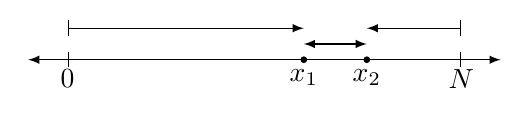
\begin{tikzpicture}
        \draw[latex-latex] (-3,0) -- (3,0);
        \draw[|-|] (-2.5,0) node[below] {$0$} -- (2.5,0) node[below] {$N$};
        %\draw[|-|] (-2.5,-0.5) -- node[below] {$N$} (2.5,-0.5);
        \filldraw (0.5,0) circle (1pt) node[below] {$x_1$};
        \filldraw (1.3,0) circle (1pt) node[below] {$x_2$};
        \draw[latex-latex] (0.5,0.2) -- (1.3,0.2);
        \draw[latex-|] (1.3,0.4) -- (2.5,0.4);
        \draw[|-latex] (-2.5,0.4) -- (0.5,0.4);
    \end{tikzpicture}
    \caption{A one-dimensional diagram of toroidal distance, with the two arrows representing two possible distances}%
    \label{fig:2distanceexample}
\end{figure}


To obtain a general equation which works with both $x_1>x_2$ and $x_1<x_2$ (as we cannot assume $x_1<x_2$), we can write
\begin{align*}
    \Delta_1(x)&=\lvert x_2-x_1 \rvert \\
    \Delta_2(x)&=\min{(x_1,x_2)}+N-\max{(x_1,x_2)}
    %\label{eq:absoluteToroidDistance}
\end{align*}
where $\lvert a\rvert$ is the absolute value of $a$, $\min{(a,b)}$ and $\max{(a,b)}$ are defined as the minimum and maximum between the values of $a$ and $b$ respectively. They can be defined with piece-wise functions as follows:
\begin{align*}
        \min{(a,b)}=
        \begin{cases}
            a&\text{if $a\leq b$}\\
            b&\text{if $a>b$}\\
        \end{cases}\qquad
        \max{(a,b)}=
        \begin{cases}
            a&\text{if $a\geq b$}\\
            b&\text{if $a<b$}\\
        \end{cases}
    %\label{eq:}
\end{align*}
$\min$ and $\max$ are used to determine the  ``left-most'' and the ``right-most'' numbers.

Since the distance can only have one value, it is defined as the minimum of the two possible distances:
\begin{align*}
    \Delta x=\min{(\Delta_1(x),\Delta_2(x))}
\end{align*}

Generalizing it to 2 dimensions, we get
\begin{align*}
    d(s_1,s_2)&=\sqrt{(\Delta x)^2+(\Delta y)^2} \\
    d^2(s_1,s_2)&=(\Delta x)^2+(\Delta y)^2
\end{align*}
From now on, \emph{distance} refers to $d^2$.

\subsubsection{Token Comparisons}%
\label{ssub:token_comparisons}
Within this essay, a \emph{comparison} is defined as the distance between two tokens within a toroidal grid $X$. To be able to perform comparisons for every possible pair of tokens, a grid of comparisons on the grid is required. A viable approach would be to represent the comparison in a 4-dimensional grid (or tensor), where every token in the grid (first 2 dimensions), is compared to every token (next 2 dimensions). An example of the structure of the comparison for a $2\times 2$ grid is shown in \autoref{fig:4dcomparison}. The white boxes denote duplicate comparisons (eg. $
\begin{smallmatrix}
    BA\\ AA
\end{smallmatrix}
$ is identical to
$
\begin{smallmatrix}
    AA\\ BA
\end{smallmatrix}
$), because the distance is invariant to the order of the tokens.

But since removing the irregularly shaped duplicate entries is not a trivial task with a 4-dimensional representation --- especially if we extend beyond a $N=2$ grid --- we can simplify the problem by reducing the dimensionality of the grid: from an $N\times N\times N\times N$ grid to a $N^2\times N^2$ grid. The elements within the 4-dimensional matrix are in the form $C_{i,j,k,l}$, and the 2-dimensional grid in the form $C_{ij,kl}$, but both represent the same thing: a the distance between the tokens $\bm{IJ}$ and $\bm{KL}$. The two-dimensional representation of \autoref{fig:4dcomparison} is shown in \autoref{fig:2dcomparison}. By doing so, we can easily remove the duplicate entries by multiplying it with an upper triangular matrix, further explained in \ref{ssub:loss_function_as_matrix_multiplications}. Let $C_{2d}$ denote a function mapping from the input toroidal grid $X$ and returning the 2d-comparison grid $C_{2d}(X)$.
\begin{figure}[htpb]
    \centering
    \begin{subfigure}[t]{0.5\textwidth}
    \begin{center}
    \nestedToroid{2}
    \end{center}
    \caption{4-dimensional comparison with elements in the form $C(X)_{i,j,k,l}$}
    \label{fig:4dcomparison}
    \end{subfigure}%
    ~
    \begin{subfigure}[t]{0.5\textwidth}
    \begin{center}
    \twodcomparison{2}
    \end{center}
    \caption{2-dimensional comparison with elements in the form $C(X)_{ij,kl}$}
    \label{fig:2dcomparison}
    \end{subfigure}

    \caption{Tensors $C(X)$ representing comparison grids of a $2\times 2$ toroidal grid, where every element represents the distance between $X_{ij}$ and $X_{kl}$. Shaded cells denote unique comparisons.}%
    \label{fig:comparisonGrids}
\end{figure}

\subsubsection{Loss Function as Matrix Multiplications}%
\label{ssub:loss_function_as_matrix_multiplications}
Let $\odot$ denote the element-wise matrix multiplication
(eg.~$
\begin{psmallmatrix}
    a&b\\
    c&d
\end{psmallmatrix}\odot
\begin{psmallmatrix}
    e&f\\
    g&h
\end{psmallmatrix}=
\begin{psmallmatrix}
    a\cdot e&b\cdot f\\
    c\cdot g&d\cdot h
\end{psmallmatrix}
$), and $O$ denotes the original grid. The loss function for toroidal grid $X$ is equal to
\begin{align*}
    L(x)&=\sum_i^{N^2}\sum_j^{N^2}C(X)_{ij}C(O)_{ij}U_{ij}\\
        &=\sum C(X)\odot C(O)\odot U
\end{align*}
where $C(X),C(O),\text{ and }U$ are matrices of the form $N^2\times N^2$, and $U_{ij}$ is defined with the piece-wise defined function:
\begin{align*}
    U_{ij}=
    \begin{cases}
        1, & j\geq i \\
        0, & j<i
    \end{cases}
\end{align*}
an example the matrix $U$ with shape $4\times 4$ is as follows:
 \begin{align*}
    \begin{bmatrix}
        1&1&1&1\\
        0&1&1&1\\
        0&0&1&1\\
        0&0&0&1
    \end{bmatrix}
\end{align*}
Multiplying by $U$ has the effect of removing duplicate comparisons, satisfying our requirement of measuring only unique pairs of tokens.
